\chapter{Datasets statistics}

\begin{figure}[hbt]
  \centering
  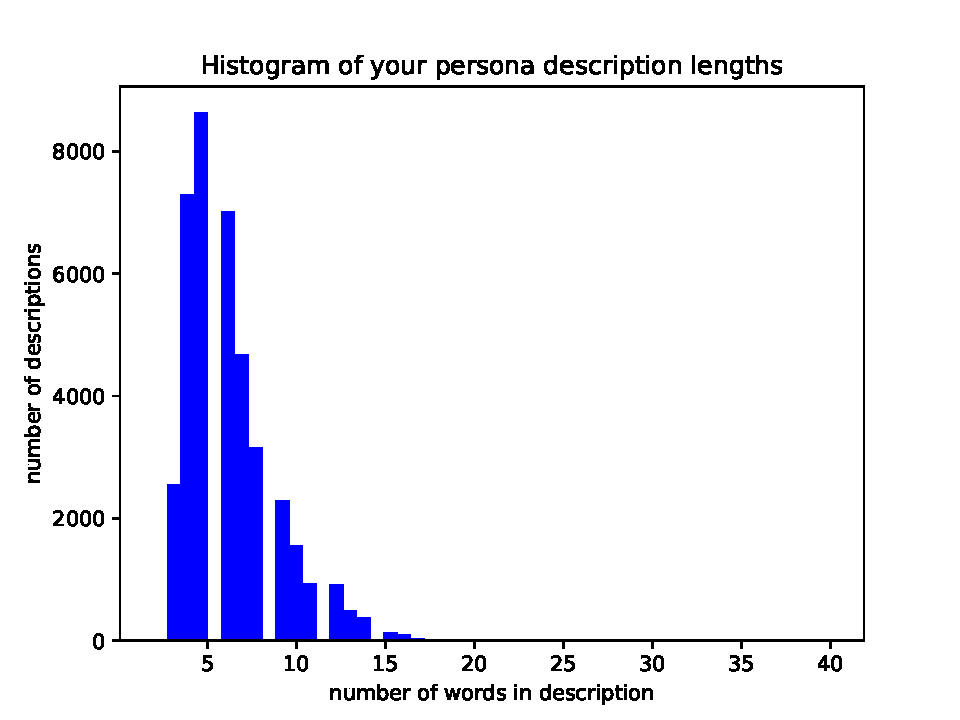
\includegraphics[width=0.7\textwidth]{figures/persona_desc.pdf}
  \caption{Histogram of persona description lengths.}
  \label{fig:histogram_persona_desc}
\end{figure}

\begin{figure}[hbt]
  \centering
  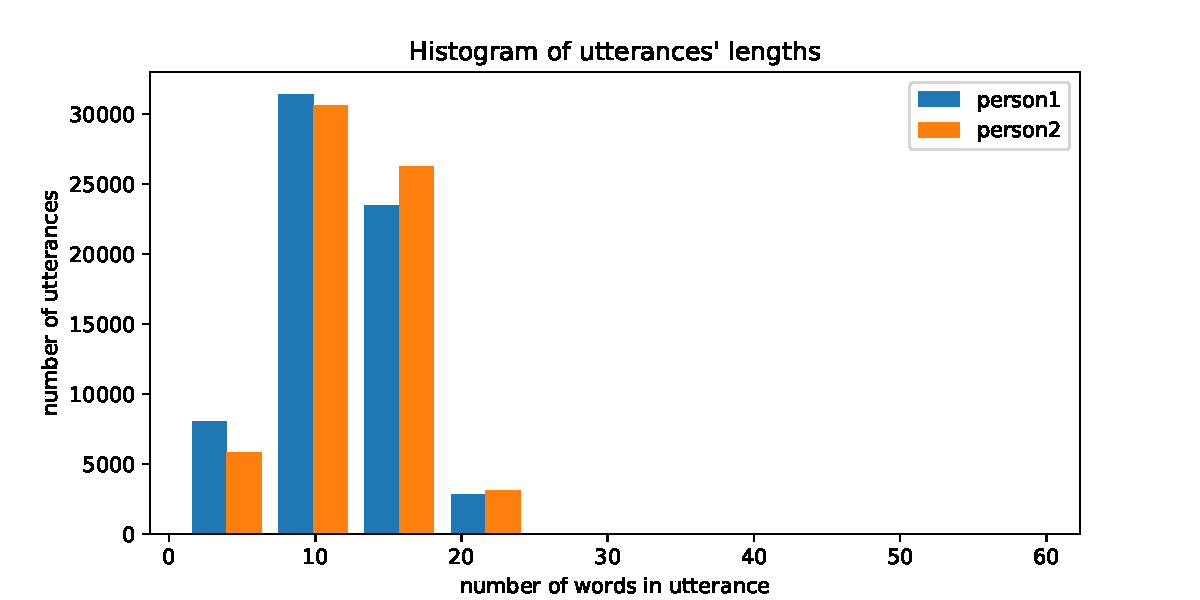
\includegraphics[width=0.7\textwidth]{figures/uttr_length.pdf}
  \caption{Histogram of utterances' lengths of a person.}
  \label{fig:histogram_uttr_length}
\end{figure}

\begin{figure}
  \centering
  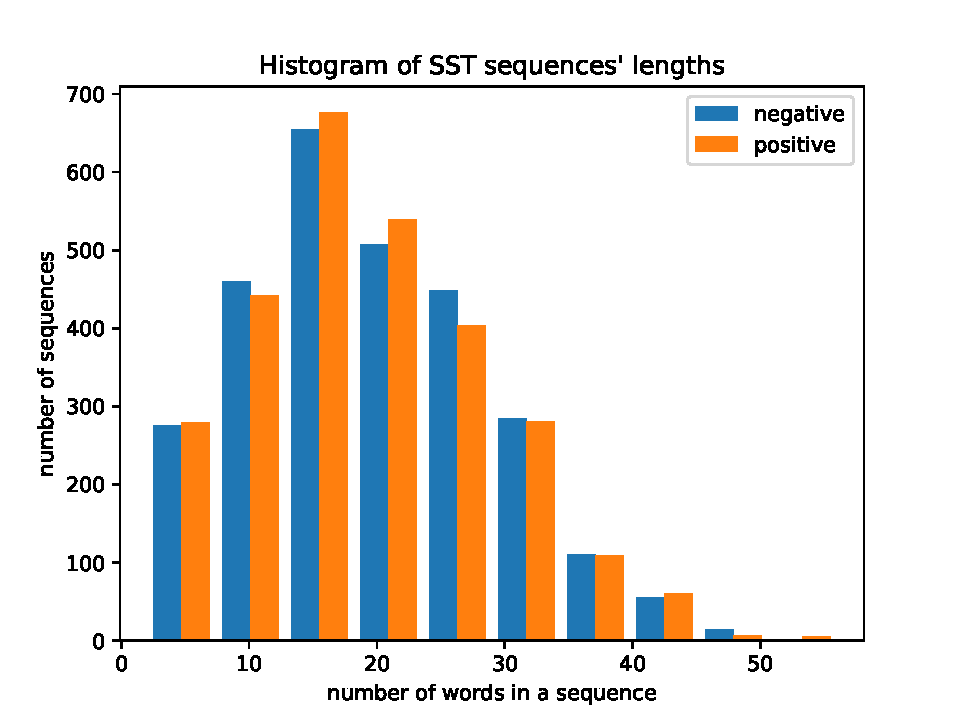
\includegraphics[width=0.7\textwidth]{figures/sst.pdf}
  \caption{Histogram of Stanford Sentiment Treebank labeled reviews.}
  \label{fig:sst}
\end{figure}

\begin{figure}
  \centering
  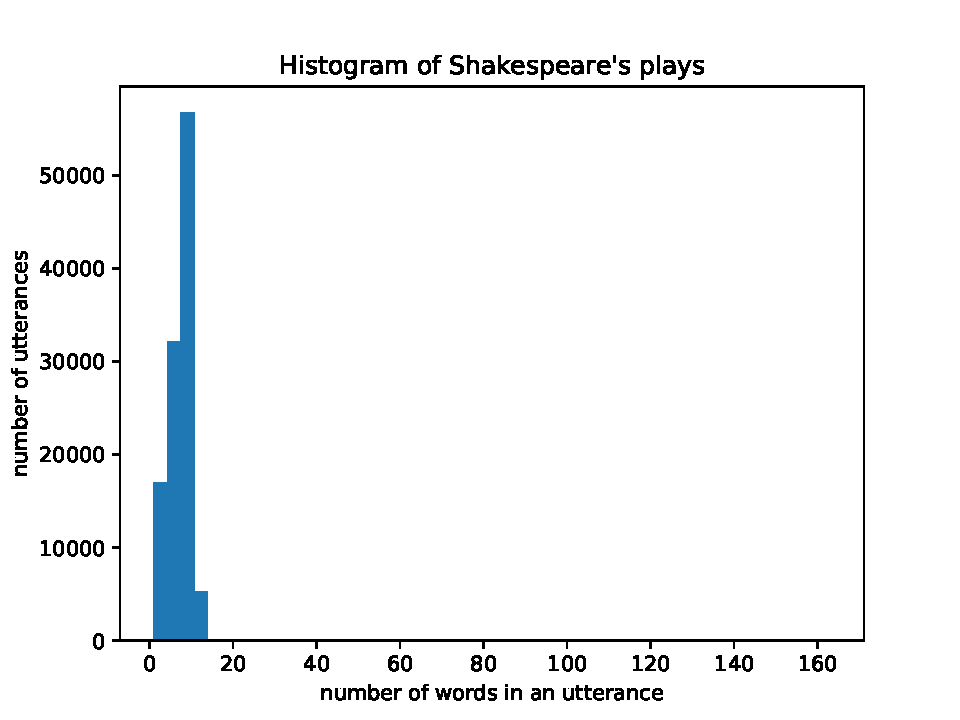
\includegraphics[width=0.7\textwidth]{figures/shakespeare.pdf}
  \caption{Histogram of Shakespeare's plays.}
  \label{fig:shakespeare}
\end{figure}

\begin{figure}[hbt]
  \centering
  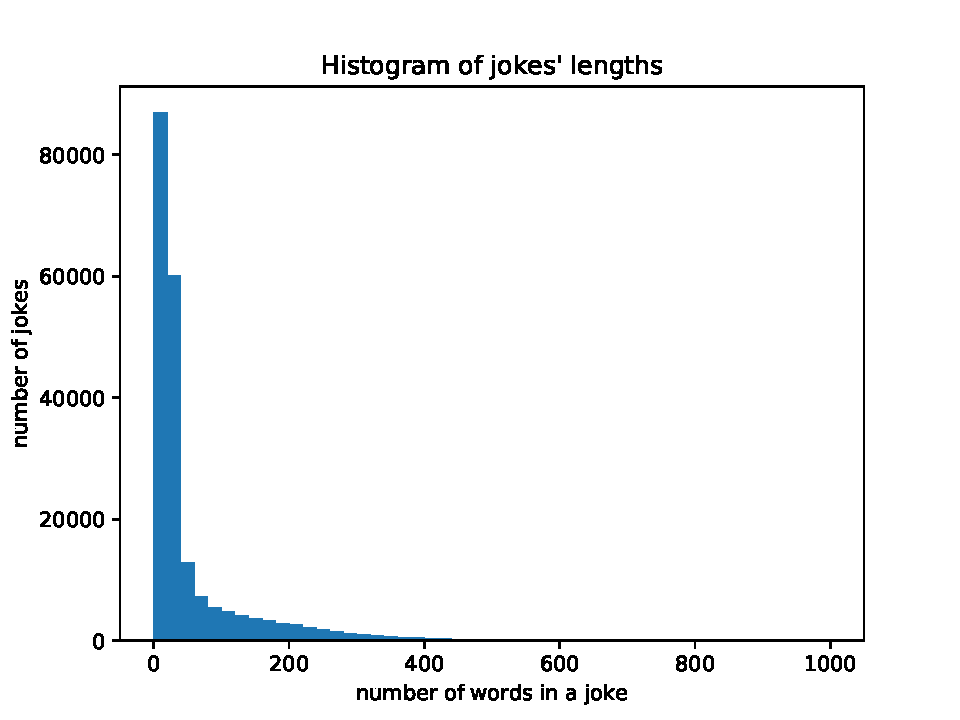
\includegraphics[width=0.7\textwidth]{figures/jokes.pdf}
  \caption{Histogram of jokes lengths.}
  \label{fig:jokes}
\end{figure}

\begin{figure}[hbt]
  \centering
  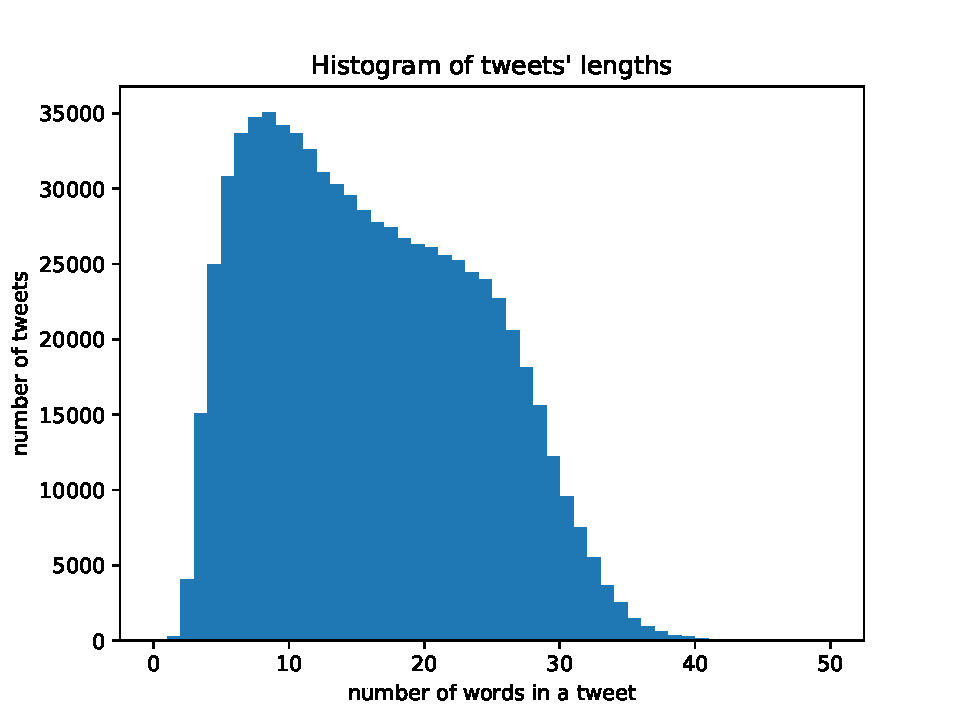
\includegraphics[width=0.7\textwidth]{figures/tweet.pdf}
  \caption{Histogram of tweets' lengths.}
  \label{fig:tweet}
\end{figure}

\chapter{Luong attention} \label{luong_attn_appendix}

Information in this chapter is taken from \cite{luong2015effective}.
\begin{figure}[hbt]
  \centering
  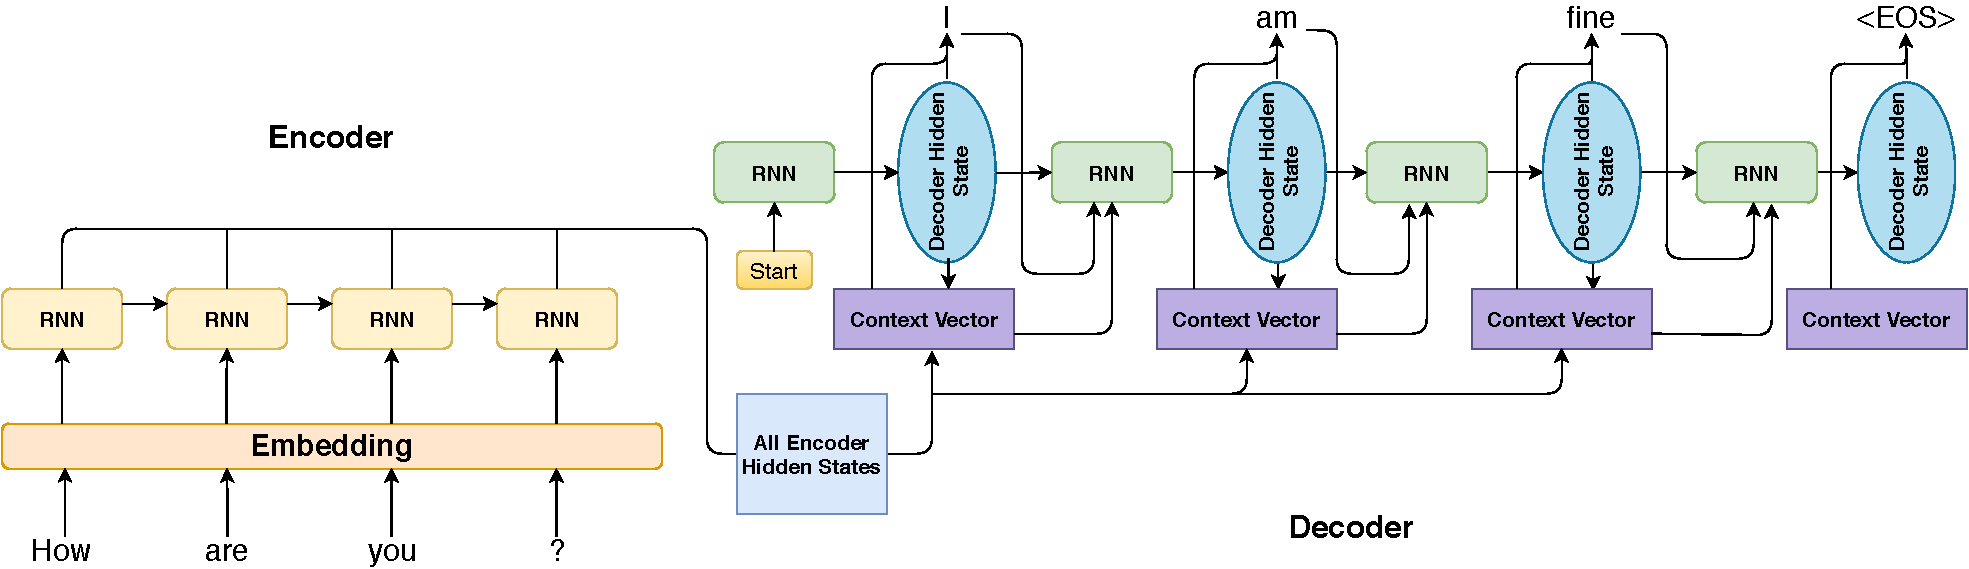
\includegraphics[width=1\textwidth]{figures/luong_decoder.pdf}
  \caption{Luong decoder architecture.}
  \label{luong}
\end{figure}

Luong attention model is classified into 2 categories, \textit{global} and \textit{local}. Common to these types of model is the fact that at each time step \textit{t} in the decoding phase previous hidden state is taken as input to derive a context vector $\mathbf{c_t}$, that captures relevant information to predict the current target word $y_t$. This categories differ only if ``attention'' is placed on all source positions or on a few source positions.

The simple concatenation layer combines the information from vectors $h_t$ and $c_t$ to produce an attentional hidden state (Equation \ref{eq:hs}).
\begin{equation} \label{eq:hs}
\mathbf{\widetilde{h_t}} = tanh(\mathbf{W_c}[\mathbf{c_t};\mathbf{h_t}])
\end{equation}

The attention vector $\mathbf{\widetilde{h_t}}$ then passed through the softmax layer to produce the predictive distribution (Equation \ref{eq:sfm}).
\begin{equation} \label{eq:sfm}
p(y_t|y_{<t},x) = softmax(\mathbf{W_s}\mathbf{\widetilde{h_t}})
\end{equation}

\subsubsection{Global Attention}
An alignment vector $a_t$ (size of $a_t$ is equal to the number of time steps on the source side) is derived by comparing the current target hidden state $\mathbf{h_t}$ with each source hidden state $\mathbf{\bar{h}_s}$ (Equation \ref{eq:av}).
\begin{equation} \label{eq:av}
a_t(s) = align(\mathbf{h_t}, \mathbf{\bar{h}_s}) = \frac{exp(score(\mathbf{h_t}, \mathbf{\bar{h}_s}))}{\sum_{s'} exp(score(\mathbf{h_t}, \mathbf{\bar{h}_s}))}
\end{equation}

There are three types of the score function (the score function is referred as a content-based function) (Equation \ref{eq:sf}).
\begin{equation}\label{eq:sf}
score(\mathbf{h_t}, \mathbf{\bar{h}_s}) = \begin{cases} \mathbf{h_t}^\intercal \mathbf{\bar{h}_s}, & \mbox{dot} \\ \mathbf{h_t}^\intercal \mathbf{W_a} \mathbf{\bar{h}_s}, & \mbox{general} \\ \mathbf{v_a}^\intercal tanh(\mathbf{W_a} [\mathbf{h_t}; \mathbf{\bar{h}_s}]), & \mbox{concat} \end{cases}
\end{equation}

In location-based function the alignment scores are computed from solely the target hidden state $\mathbf{h_t}$ (Equation \ref{eq:sfm_as}).
\begin{equation} \label{eq:sfm_as}
a_t = softmax(\mathbf{W_a}\mathbf{h_t})
\end{equation}

The context vector $\mathbf{c_t}$ is computed as the weighted average over all the source hidden state, where alignment vector represents weights.

\subsubsection{Local Attention}
Global attention is expensive, because it has to attend to all words on the source side for each target word. Local attention chooses to focus only on a small subset of the source positions per target word.

The local alignment vector $a_t$ in this category of attention is fixed-dimensional, because of it there are 2 variants of the model, \textit{monotonic} (Equation \ref{eq:monotonic}) and \textit{predictive} (Equation \ref{eq:predictive}).

\begin{equation} \label{eq:monotonic}
p_t = t
\end{equation}

\begin{equation} \label{eq:predictive}
p_t = S \cdot sigmoid(\mathbf{v_p}^\intercal tanh(\mathbf{W_p} \mathbf{h_t}))
\end{equation}

In monotonic alignment the source and target sequences are roughly monotonically aligned. In predictive alignment the model learns to predict the alignment position, where $\mathbf{W_p}$ and $\mathbf{v_p}$ are the learned model parameters.

Gaussian distribution centered in $p_t$ is used to favor alignment points near $p_t$ (Equation \ref{eq:align_gaus}).
\begin{equation} \label{eq:align_gaus}
a_t(s) = align(\mathbf{h_t}, \mathbf{\bar{h}_s}) exp(-\frac{(s-p_t)^2}{2\sigma^2})
\end{equation}

